\chapter{Simulation Results}
\label{chap:results}

\section{Programming Environment}
\label{sec:environment}

Simulations were carried out using the foam-extend 4.0 fork of the OpenFOAM (Open-Source Field Operation And Manipulation) software project. OpenFOAM was selected as it is a mature and feature rich platform for computational fluid dynamics, and thus already provides many utilities and functionality for tasks such as pre- and post-processing data, run time slection of simulation parameters, and managing very generic mesh structures. It is coded almost entirely in object-oriented C++, making it very flexible for extension, although at over one million lines of code it is still a far from simple endeavour.

The foam-extend fork was chosen over the standard OpenFOAM distribution as it includes an additional density-basesd Navier Stokes (DBNS) solver which implements very closely the basic FVM method which was to be modified. As well, this DBNS library contains several already programmed numerical fluxes and gradient limiters, such that the focus could remain on developing the well-balanced reconstruction without having to code all of the supporting pieces from scratch.


\section{Order Verification Study}
\label{sec:OVS}

An order verification study (OVS) was carried out to verify that the implementation matched the theoretically expected convergence rates. For the tests, a piecewise continuous potential function defined on the 1D domain from $y=-2$ to $y=2$ was used, composed of two small constant regions at the boundaries connected by a fifth-order polynomial,
\begin{equation}
\phi(y)=
\begin{dcases} 
      0, & y\leq -1.5 \\
      \frac{2}{81}y^5+\frac{5}{27}y^3+\frac{5}{8}y+\frac{1}{2}, & -1.5<y<1.5 \\
      1, & y\geq 1.5
\end{dcases}.
\end{equation}
The constant regions at the domain edges allowed for simple zero-gradient boundary conditions to be used for all non-fixed, and the quintic coefficients were chosen to also match the first and second derivatives at the transition points to the constant regions.

The inlet of the flow was set using dirichlet boundary conditions on $T$ and $\textrm{v}_y$ at $y=2$ with the primitve values the same as used for the inlet for the sub-problem 2 described in section~\ref{subsec:sub_problem_1}; see there for a more detailed description of how these values are determined. To briefly summarize here, at the inlet one has $p=0.75, T=1.05,$ and $\textrm{v}_y=-\sqrt{31/199}$, with adiabatic constant $\gamma=4/3$ and units such that $c=1$ and $\rho=1$. The inlet condition for the pressure is set to zero-gradient at the inlet, as having both it and the velocity fixed caused spurious error in some test cases and was recommended against in the OpenFOAM documenation. At the outlet, all primitives were given homogenous Neumann boundary conditions.

For the initial conditions in the rest of the domain, the value of the density $\rho(y)$ for a flow equilibrium flow was calculated, and then superimposed with a Gaussian perturbation centred at $y=0$, given by
\begin{equation}
\Delta \rho(y)=\frac{A}{2\sigma \sqrt{2 \pi}}\ \textrm{exp}\left[-\frac{1}{2}\left(\frac{y}{\sigma}\right)^2\right].
\end{equation}
The width of the Gaussian was determined with $\sigma=0.2$ and the amplitude $A$ was varied to control the maximal magnitude of the perturbation over several series of tests.

Results of the simulations are characterized using the normalized L1 norm of the error
\begin{equation}
Err_1=\frac{1}{N}\sum\limits_{i=1}^N \left|\rho_i-\rho_{i,\textrm{ref}}\right|,
\end{equation}
where $\rho_{\textrm{ref}}$ is a reference solution that is obtained either from exact calculation of the unperturbed equilibrium flow values, or from an overkill high-resolution simulation computed using $N=12800$ cells and the second-order well-balanced scheme for the test cases with the Gaussian perturbation. For the OVS, the number of cells is progressivley doubled from $N=25$ to $N=6400$ and the single-step order of accuracy is computed by determinig the slope of the line connecting the error values of each adjacent pair of simulations on a log-log plot of $Err_1$ vs.\ $\Delta y$, the grid spacing.

\begin{table*}\centering
\caption{L1 error and order of accuracy for the first- and second-order unbalanced/well-balanced schemes with no perturbation, i.e.\ $A=0$.}
\ra{1.3}
\label{table:OVS_A0}
\begin{tabular}{@{}rcccccc@{}}\toprule
& \phantom{a} & \multicolumn{2}{c}{First} & \phantom{ab} & \multicolumn{2}{c}{Second}\\
\cmidrule{3-4} \cmidrule{6-7}
$N$ && $Err_1$ & Order && $Err_1$ & Order\\ \midrule
$25$ && 3.47e-02/4.40e-15 &&& 4.51e-03/4.40e-15 &\\
$50$ && 1.75e-02/4.37e-15 & 0.987/- && 1.12e-03/4.37e-15 & 2.013/-\\
$100$ && 8.79e-03/4.16e-15 & 0.993/- && 2.77e-04/4.16e-15 & 2.013/-\\
$200$ && 4.41e-03/3.15e-15 & 0.996/- && 6.88e-05/3.35e-15 & 2.009/-\\
$400$ && 2.21e-03/3.48e-15 & 0.998/- && 1.71e-05/3.46e-15 & 2.004/-\\
$800$ && 1.10e-03/2.88e-15 & 0.999/- && 4.28e-06/2.96e-15 & 2.003/-\\
$1600$ && 5.53e-04/3.05e-14 & 1.000/- && 1.07e-06/6.83e-14 & 2.002/-\\
$3200$ && 2.76e-04/1.02e-13 & 1.000/- && 2.67e-07/1.20e-13 & 2.001/-\\
$6400$ && 1.38e-04/7.80e-14 & 1.000/- && 6.67e-08/8.56e-14 & 2.000/-\\
\bottomrule
\end{tabular}
\end{table*}

\begin{table*}\centering
\caption{L1 error and order of accuracy for the first- and second-order unbalanced/well-balanced schemes with medium perturbation amplitude $A=0.1$.}
\ra{1.3}
\label{table:OVS_Amedium}
\begin{tabular}{@{}rcccccc@{}}\toprule
& \phantom{a} & \multicolumn{2}{c}{First} & \phantom{ab} & \multicolumn{2}{c}{Second}\\
\cmidrule{3-4} \cmidrule{6-7}
$N$ && $Err_1$ & Order && $Err_1$ & Order\\ \midrule
$25$ && 3.46e-02/1.04e-02 &&& 6.97e-03/4.55e-03 &\\
$50$ && 1.77e-02/7.69e-03 & 0.96/0.44 && 2.30e-03/1.62e-03 & 1.60/1.49\\
$100$ && 9.55e-03/5.27e-03 & 0.89/0.55 && 5.83e-04/4.62e-04 & 1.98/1.81\\
$200$ && 5.22e-03/3.29e-03 & 0.87/0.68 && 1.36e-04/1.10e-04 & 2.10/2.07\\
$400$ && 2.83e-03/1.89e-03 & 0.88/0.80 && 3.31e-05/2.69e-05 & 2.03/2.03\\
$800$ && 1.49e-03/1.02e-03 & 0.92/0.88 && 8.75e-06/6.46e-06 & 1.92/2.06\\
$1600$ && 7.71e-04/5.36e-04 & 0.95/0.94 && 3.39e-06/1.62e-06 & 1.37/2.00\\
$3200$ && 3.93e-04/2.74e-04 & 0.97/0.97 && 2.62e-06/5.16e-07 & 0.37/1.65\\
$6400$ && 1.98e-04/1.39e-04 & 0.99/0.98 && 2.45e-06/3.93e-07 & 0.10/0.39\\
\bottomrule
\end{tabular}
\end{table*}

\begin{table*}\centering
\caption{L1 error and order of accuracy for the first- and second-order unbalanced/well-balanced schemes with very large perturbation amplitude $A=2$.}
\ra{1.3}
\label{table:OVS_Alarge}
\begin{tabular}{@{}rcccccc@{}}\toprule
& \phantom{a} & \multicolumn{2}{c}{First} & \phantom{ab} & \multicolumn{2}{c}{Second}\\
\cmidrule{3-4} \cmidrule{6-7}
$N$ && $Err_1$ & Order && $Err_1$ & Order\\ \midrule
$25$ && 1.68e-01/1.67e-01 &&& 6.07e-02/6.29e-02 &\\
$50$ && 1.12e-01/1.12e-01 & 0.58/0.58 && 3.06e-02/3.14e-02 & 0.99/1.00\\
$100$ && 7.46e-02/7.41e-02 & 0.59/0.60 && 1.47e-02/1.47e-02 & 1.06/1.09\\
$200$ && 4.54e-02/4.48e-02 & 0.72/0.73 && 5.86e-03/5.86e-03 & 1.32/1.33\\
$400$ && 2.69e-02/2.67e-02 & 0.76/0.75 && 3.26e-03/3.26e-03 & 0.85/0.84\\
$800$ && 1.50e-02/1.49e-02 & 0.84/0.85 && 1.40e-03/1.40e-03 & 1.22/1.22\\
$1600$ && 8.35e-03/8.25e-03 & 0.85/0.85 && 6.57e-04/6.58e-04 & 1.09/1.09\\
$3200$ && 4.57e-03/4.52e-03 & 0.87/0.87 && 3.15e-04/3.11e-04 & 1.06/1.08\\
$6400$ && 2.43e-03/2.40e-03 & 0.91/0.91 && 1.32e-04/1.23e-04 & 1.25/1.33\\
\bottomrule
\end{tabular}
\end{table*}

\begin{table*}\centering
\caption{L1 error and order of accuracy for the first- and second-order unbalanced/well-balanced schemes with very small perturbation amplitude $A=1e-4$.}
\ra{1.3}
\label{table:OVS_Asmall}
\begin{tabular}{@{}rcccccc@{}}\toprule
& \phantom{a} & \multicolumn{2}{c}{First} & \phantom{ab} & \multicolumn{2}{c}{Second}\\
\cmidrule{3-4} \cmidrule{6-7}
$N$ && $Err_1$ & Order && $Err_1$ & Order\\ \midrule
$25$ && 3.47e-02/1.05e-05 &&& 4.51e-03/4.79e-06 &\\
$50$ && 1.75e-02/7.83e-06 & 0.99/0.42 && 1.12e-03/1.76e-06 & 2.01/1.44\\
$100$ && 8.79e-03/5.39e-06 & 0.99/0.54 && 2.77e-04/4.67e-07 & 2.01/1.91\\
$200$ && 4.41e-03/3.36e-06 & 1.00/0.68 && 6.88e-05/1.10e-07 & 2.01/2.09\\
$400$ && 2.21e-03/1.93e-06 & 1.00/0.80 && 1.71e-05/2.72e-08 & 2.00/2.01\\
$800$ && 1.10e-03/1.05e-06 & 1.00/0.88 && 4.28e-06/6.63e-09 & 2.00/2.04\\
$1600$ && 5.53e-04/5.49e-07 & 1.00/0.94 && 1.07e-06/1.64e-09 & 2.00/2.01\\
$3200$ && 2.76e-04/2.81e-07 & 1.00/0.97 && 2.68e-07/5.12e-10 & 2.00/1.68\\
$6400$ && 1.38e-04/1.42e-07 & 1.00/0.98 && 6.80e-08/3.83e-10 & 1.98/0.42\\
\bottomrule
\end{tabular}
\end{table*}


\section{Toy Problem}
\label{sec:toyProblem}

As mentioned at the beginning of chapter~\ref{chap:introduction}, the simple toy model of FS~\cite{Foglizzo2009,Sato2009} was chosen as a useful initial application of our well-balanced method to the SASI. The salient details from those papers  are reproduced here. Following the notation of FS, we will denote quantities in the supersonic region before the shock with a subscript `1', in the interior region between the shock and potential step with `in', and in the outflow region past the step with `out'.

A schematic view of the problem domain can be seen in Fig.~\ref{fig:Sato1}, showing how the overall scenario is split into two sub-problems for simulation. The entire test case consists of an supersonic inflow deccelerated at a stationary shock front, followed shortly after by a potential step which further slows the now subsonic flow. This provides a very simplistic analogue to study the mechanisms at play during the inflow, decceleration, and accretion of matter in a collapsing star before supernova.

\begin {figure}
\centering
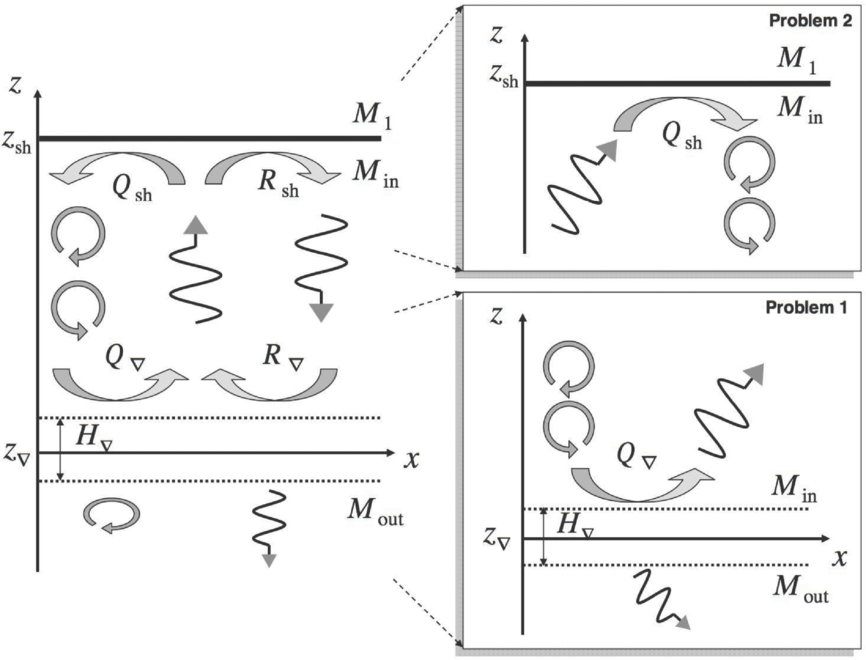
\includegraphics[width=13cm]{figures/Sato1}
\caption {A short caption.}
\label{fig:Sato1}
\end{figure}

For ease of simulation, the potential step and stationary shock are computed separately as sub-problems 1 and 2 respectively. This separation greatly simplifies the introduciton of specific advective and acoustic pertubations to appropriate locations in the interior of the domain, making it much easier to see the interactions of these disturbances at the boundaries (the shock and potential step) between the various flow regions.

\subsection{Sub-Problem 1}
\label{subsec:sub_problem_1}

A hyperbolic tangent function is used to provide a smooth step-like external potential field, with the exact function given by
\begin{equation}
\phi(x)=\frac{\Delta \phi}{2}\left[\textrm{tanh}\left(\frac{y-y_{\nabla}}{H_{\nabla}/2}\right)+1\right],\quad x\in[-2,2],
\end{equation}
where the step size $\Delta \phi$ is set based on the ratio of the sound speeds $c_{\textrm{in}}/c_{\textrm{out}}$ in the constant regions surrounding the step.

\subsection{Sub-Problem 2}

Description of the standing shock